% Options for packages loaded elsewhere
\PassOptionsToPackage{unicode}{hyperref}
\PassOptionsToPackage{hyphens}{url}
%
\documentclass[
]{article}
\usepackage{amsmath,amssymb}
\usepackage{lmodern}
\usepackage{iftex}
\ifPDFTeX
  \usepackage[T1]{fontenc}
  \usepackage[utf8]{inputenc}
  \usepackage{textcomp} % provide euro and other symbols
\else % if luatex or xetex
  \usepackage{unicode-math}
  \defaultfontfeatures{Scale=MatchLowercase}
  \defaultfontfeatures[\rmfamily]{Ligatures=TeX,Scale=1}
\fi
% Use upquote if available, for straight quotes in verbatim environments
\IfFileExists{upquote.sty}{\usepackage{upquote}}{}
\IfFileExists{microtype.sty}{% use microtype if available
  \usepackage[]{microtype}
  \UseMicrotypeSet[protrusion]{basicmath} % disable protrusion for tt fonts
}{}
\makeatletter
\@ifundefined{KOMAClassName}{% if non-KOMA class
  \IfFileExists{parskip.sty}{%
    \usepackage{parskip}
  }{% else
    \setlength{\parindent}{0pt}
    \setlength{\parskip}{6pt plus 2pt minus 1pt}}
}{% if KOMA class
  \KOMAoptions{parskip=half}}
\makeatother
\usepackage{xcolor}
\usepackage[margin=1in]{geometry}
\usepackage{graphicx}
\makeatletter
\def\maxwidth{\ifdim\Gin@nat@width>\linewidth\linewidth\else\Gin@nat@width\fi}
\def\maxheight{\ifdim\Gin@nat@height>\textheight\textheight\else\Gin@nat@height\fi}
\makeatother
% Scale images if necessary, so that they will not overflow the page
% margins by default, and it is still possible to overwrite the defaults
% using explicit options in \includegraphics[width, height, ...]{}
\setkeys{Gin}{width=\maxwidth,height=\maxheight,keepaspectratio}
% Set default figure placement to htbp
\makeatletter
\def\fps@figure{htbp}
\makeatother
\setlength{\emergencystretch}{3em} % prevent overfull lines
\providecommand{\tightlist}{%
  \setlength{\itemsep}{0pt}\setlength{\parskip}{0pt}}
\setcounter{secnumdepth}{-\maxdimen} % remove section numbering
\usepackage{amsmath}
\usepackage{booktabs}
\usepackage{caption}
\usepackage{longtable}
\ifLuaTeX
  \usepackage{selnolig}  % disable illegal ligatures
\fi
\IfFileExists{bookmark.sty}{\usepackage{bookmark}}{\usepackage{hyperref}}
\IfFileExists{xurl.sty}{\usepackage{xurl}}{} % add URL line breaks if available
\urlstyle{same} % disable monospaced font for URLs
\hypersetup{
  pdftitle={simulation-plots},
  pdfauthor={Leonardo Feitosa},
  hidelinks,
  pdfcreator={LaTeX via pandoc}}

\title{simulation-plots}
\author{Leonardo Feitosa}
\date{2023-02-24}

\begin{document}
\maketitle

\begin{verbatim}
## # A tibble: 1,302 x 19
##    scenario_id   p_s   p_w   r_s   r_w   q_s   q_w   k_s   k_w     c variables
##          <dbl> <dbl> <dbl> <dbl> <dbl> <dbl> <dbl> <dbl> <dbl> <dbl> <chr>    
##  1          53   0.5     0   0.2  0.1   0.05  0.05     4     2  0.05 N_w      
##  2         252   0.3     0   0.6  0.1   0.05  0.05     4     2  0.05 N_w      
##  3         553   0.5     0   0.2  0.11  0.05  0.05     4     2  0.05 N_w      
##  4         752   0.3     0   0.6  0.11  0.05  0.05     4     2  0.05 N_w      
##  5        1302   0.3     0   0.7  0.12  0.05  0.05     4     2  0.05 N_w      
##  6        1554   0.7     0   0.2  0.13  0.05  0.05     4     2  0.05 N_w      
##  7        2054   0.7     0   0.2  0.14  0.05  0.05     4     2  0.05 N_w      
##  8        2352   0.3     0   0.8  0.14  0.05  0.05     4     2  0.05 N_w      
##  9        2555   0.9     0   0.2  0.15  0.05  0.05     4     2  0.05 N_w      
## 10        2603   0.5     0   0.3  0.15  0.05  0.05     4     2  0.05 N_w      
## # ... with 1,292 more rows, and 8 more variables: values <dbl>, b_stocks <chr>,
## #   b_v_k <dbl>, vuln_ratio_w <dbl>, vuln_ratio_s <dbl>, st_stock_rev <dbl>,
## #   w_stock_rev <dbl>, mean_ps <dbl>
\end{verbatim}

\hypertarget{results-from-the-parameter-per-parameter-simulation}{%
\section{Results from the parameter per parameter
simulation}\label{results-from-the-parameter-per-parameter-simulation}}

\hypertarget{model-equations}{%
\subsection{Model equations:}\label{model-equations}}

\begin{itemize}
\tightlist
\item
  Strong stock size (\(N_s\))
\end{itemize}

\[
\frac{dN_s}{N_wdt} = r_s (1 - \frac{N_s}{K_s}) - q_s E
\]

\begin{itemize}
\tightlist
\item
  Weak stock size (\(N_w\)):
\end{itemize}

\[
\frac{dN_w}{N_wdt} = r_w (1 - \frac{N_w}{K_w}) - q_w E
\]

\begin{itemize}
\tightlist
\item
  Effort (\(E\)):
\end{itemize}

\[
\frac{dE}{Edt} = (p_s q_s N_s + p_w q_w N_w) - C
\]

\hypertarget{equilibrium-points-for-the-three-variables}{%
\subsection{Equilibrium points for the three
variables:}\label{equilibrium-points-for-the-three-variables}}

\begin{itemize}
\tightlist
\item
  Strong stock (\(N_s\)):
\end{itemize}

\[
N_s = \frac{K_s * (c * q_s * r_w + K_w * p_w * q_w * (q_w * r_s - q_s * r_w))} {(K_w * p_w * q_w^2 * r_s + K_s * p_s * q_s^2 * r_w)}
\]

\begin{itemize}
\tightlist
\item
  Weak stock (\(N_w\)):
\end{itemize}

\[
N_w = \frac{K_w * (c * q_w * r_s + K_s * p_s * q_s * (- q_w * r_s + q_s * r_w))} {(K_w * p_w * q_w^2 * r_s + K_s * p_s * q_s^2 * r_w)}
\]

\begin{itemize}
\tightlist
\item
  Effort (\(E\)):
\end{itemize}

\[
E = \frac{(-c + K_s * p_s * q_s + K_w * p_w * q_w) * r_s * r_w} {K_w * p_w * q_w^2 r_s + K_s * p_s * q_s^2 * r_w}
\]

\hypertarget{list-of-parameters}{%
\subsubsection{List of parameters:}\label{list-of-parameters}}

\begin{itemize}
\tightlist
\item
  K = carrying capacity
\item
  r = per capita growth rate
\item
  q = catchability of stocks
\item
  c = cost of fishing
\item
  p = price
\end{itemize}

\hypertarget{parameter-space-for-both-species}{%
\subsubsection{Parameter space for both
species:}\label{parameter-space-for-both-species}}

\begin{itemize}
\tightlist
\item
  Catchability (q) varies from 0.1 to 0.5 at intervals of 0.2 for both
  species.
\item
  Growth rate (r) varies from 0.35 to 1.05 at intervals of 0.35 for the
  strong stock and from 0.1 to 0.3 at intervals of 0.1 for the weak
  stock.
\item
  Carrying capacity (k) varies from 3 to 5 at intervals of 1 for the
  strong stock and from 1 to 3 at intervals of 1 for the weak stock.
\item
  Price ranges (p) from 0.1 to 10 at intervals of 0.5 for both species.
\end{itemize}

\hypertarget{catchability-range-simulation}{%
\subsubsection{Catchability range
simulation}\label{catchability-range-simulation}}

\includegraphics{simulation-plots_files/figure-latex/unnamed-chunk-4-1.pdf}

\hypertarget{growth-range-simulation}{%
\subsubsection{Growth range simulation}\label{growth-range-simulation}}

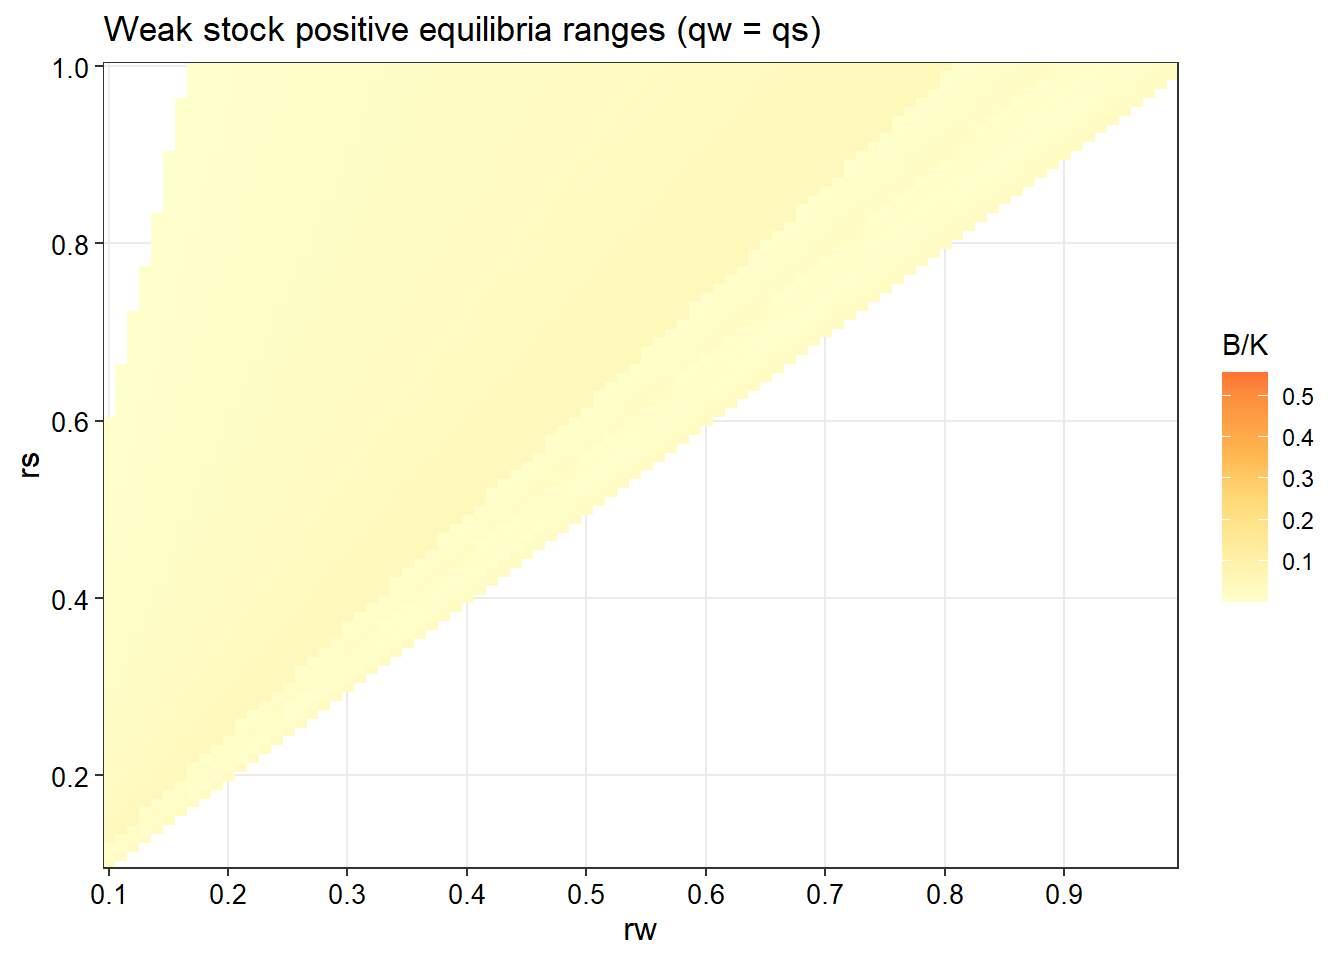
\includegraphics{simulation-plots_files/figure-latex/distribution of negative values for Ns and Nw for the range of rs-1.pdf}

\hypertarget{first-test-plot-with-weak-stock-having-zero-price}{%
\subsubsection{First test plot with weak stock having zero
price}\label{first-test-plot-with-weak-stock-having-zero-price}}

\hypertarget{vulnerability-ratios-vs-revenue-stream-with-prices-as-constants}{%
\subsubsection{Vulnerability ratios vs revenue stream with prices as
constants}\label{vulnerability-ratios-vs-revenue-stream-with-prices-as-constants}}

\begin{itemize}
\tightlist
\item
  in the top plots, \(p_w\) = 1
\item
  in the bottom plots, \(p_s\) = 1
\end{itemize}

\includegraphics{simulation-plots_files/figure-latex/unnamed-chunk-11-1.pdf}

\hypertarget{vulnerability-ratios-vs-revenue-stream-with-prices-as-functions-of-catch}{%
\subsubsection{Vulnerability ratios vs revenue stream with prices as
functions of
catch}\label{vulnerability-ratios-vs-revenue-stream-with-prices-as-functions-of-catch}}

\begin{itemize}
\tightlist
\item
  in the top plots, \(p_s\) is a parameter and \(p_w\) is a variable
\item
  in the bottom plots, \(p_w\) is a parameter and \(p_s\) is a variable
\end{itemize}

\includegraphics{simulation-plots_files/figure-latex/unnamed-chunk-15-1.pdf}

\hypertarget{time-series-equations}{%
\subsection{Time series equations}\label{time-series-equations}}

\[
\begin{align}
\frac{d N_s}{dt} &= N_S  r_s  (1 - (\frac{N_S}{K_s})) - q_s E \\
\newline
\frac{d N_w}{dt} &= N_W  r_w  (1 - (\frac{N_W}{K_w})) - q_w E \\
\newline
\frac{d E}{dt} &= \alpha  E  (p_s  q_s  N_S + p_w q_w N_W - c)
\newline
\frac{d C_s}{dt} &= q_s N_s E
\newline
\frac{d C_w}{dt} &= q_w N_w E
\newline
\frac{d CPUE_s}{dt} &= \frac{C_s} {E}
\newline
\frac{d CPUE_w}{dt} &= \frac{C_w} {E}
\newline
\frac{d \pi_s}{dt} &= C_s p_s - C_s  c
\newline
\frac{d \pi_w}{dt} &= C_w p_W - C_w  c
\newline
\frac{d \pi}{dt} &= C_s  p_s + C_w  p_w - (C_s + C_w) * c
\end{align}
\]

where \(q_s\) and \(q_w\) are the catchability of the strong and the
weak stock, respectively; \(r_s\) and \(r_w\) are the intrinsic growth
rates of the strong and weak stocks, respectively; \(p_s\) and \(p_w\)
are the prices of the strong and weak stocks, respectively; \(k_s\) and
\(k_w\) are the carrying capacities of the strong and weak stocks,
respectively; \(c\) is the fishing cost, and \(\alpha\) is a constant
controling for the speed at which effort changes following price
changes.

\hypertarget{scenarios-for-a-range-of-price-ratios}{%
\subsubsection{Scenarios for a range of price
ratios}\label{scenarios-for-a-range-of-price-ratios}}

\captionsetup[table]{labelformat=empty,skip=1pt}
\begin{longtable}{ccccccccc}
\caption*{
\large Parameter space for equilibrium points\\ 
\small \\ 
} \\ 
\toprule
parameter & PR\_10 & PR\_5 & PR\_2.5 & PR\_1 & PR\_0.75 & PR\_0.5 & PR\_0.25 & PR\_0.1 \\ 
\midrule
q\_w & 0.05 & 0.05 & 0.05 & 0.05 & 0.05 & 0.05 & 0.05 & 0.05 \\ 
q\_s & 0.05 & 0.05 & 0.05 & 0.05 & 0.05 & 0.05 & 0.05 & 0.05 \\ 
k\_w & 4.00 & 4.00 & 4.00 & 4.00 & 4.00 & 4.00 & 4.00 & 4.00 \\ 
k\_s & 2.00 & 2.00 & 2.00 & 2.00 & 2.00 & 2.00 & 2.00 & 2.00 \\ 
r\_w & 1.00 & 1.00 & 1.00 & 1.00 & 1.00 & 1.00 & 1.00 & 1.00 \\ 
r\_s & 0.75 & 0.75 & 0.75 & 0.75 & 0.75 & 0.75 & 0.75 & 0.75 \\ 
p\_s & 1.00 & 1.00 & 1.00 & 1.00 & 1.00 & 1.00 & 1.00 & 1.00 \\ 
p\_w & 0.10 & 0.20 & 0.40 & 1.00 & 1.33 & 2.00 & 4.00 & 10.00 \\ 
c & 0.05 & 0.05 & 0.05 & 0.05 & 0.05 & 0.05 & 0.05 & 0.05 \\ 
\bottomrule
\end{longtable}

\includegraphics{simulation-plots_files/figure-latex/unnamed-chunk-35-1.pdf}

Panel A shows the time series dynamics for the strong and weak stocks,
and effort. Panel B shows the same data but without effort for better
comparison. Panel C shows the CPUE and catch for the strong and weak
stocks separately. Panel D shows the profits for the strong and weak
stocks, and the total profits for the fishery through time.

\textbf{Negative equilibrium points for the weak stock only occur at
high enough prices of the strong stock. If the price ratio
(\(PR = P_s/P_w\)) is smaller than 0.25, both stock have positive
equilibrium points (at a growth rate ratio (\(r_s/r_w\)) of
\textasciitilde2).}

\begin{itemize}
\tightlist
\item
  I think this figure (or a better version of it) should also go in the
  paper, because it clearly shows how effort increases a lot when we
  consider two species, and how it drives both of them to extremely low
  levels for most of the scenarios, but not all.
\end{itemize}

\hypertarget{scenarios-for-a-range-of-productivity-ratios}{%
\subsubsection{Scenarios for a range of productivity
ratios:}\label{scenarios-for-a-range-of-productivity-ratios}}

\captionsetup[table]{labelformat=empty,skip=1pt}
\begin{longtable}{ccccccc}
\caption*{
\large Parameter space for equilibrium points\\ 
\small \\ 
} \\ 
\toprule
parameter & Rw.Rs\_0.75 & Rw.Rs\_0.88 & Rw.Rs\_0.90 & Rw.Rs\_0.92 & Rw.Rs\_0.95 & Rw.Rs\_0.97 \\ 
\midrule
q\_w & 0.05 & 0.05 & 0.05 & 0.05 & 0.05 & 0.05 \\ 
q\_s & 0.05 & 0.05 & 0.05 & 0.05 & 0.05 & 0.05 \\ 
k\_w & 4.00 & 4.00 & 4.00 & 4.00 & 4.00 & 4.00 \\ 
k\_s & 2.00 & 2.00 & 2.00 & 2.00 & 2.00 & 2.00 \\ 
r\_s & 1.00 & 1.00 & 1.00 & 1.00 & 1.00 & 1.00 \\ 
r\_w & 0.75 & 0.88 & 0.90 & 0.92 & 0.95 & 0.97 \\ 
p\_w & 1.00 & 1.00 & 1.00 & 1.00 & 1.00 & 1.00 \\ 
p\_s & 1.00 & 1.00 & 1.00 & 1.00 & 1.00 & 1.00 \\ 
c & 0.05 & 0.05 & 0.05 & 0.05 & 0.05 & 0.05 \\ 
\bottomrule
\end{longtable}

\includegraphics{simulation-plots_files/figure-latex/unnamed-chunk-51-1.pdf}

\hypertarget{estimating-equilibria-for-when-both-prices-vary-as-a-function-of-their-catches}{%
\subsubsection{Estimating equilibria for when both prices vary as a
function of their
catches}\label{estimating-equilibria-for-when-both-prices-vary-as-a-function-of-their-catches}}

\hypertarget{equations}{%
\paragraph{Equations}\label{equations}}

\$\$ \begin{align}
\frac{d N_s}{dt} &= N_S  r_s  (1 - (\frac{N_S}{K_s})) - q_s N_s^\beta_s E \\

\newline
\frac{d N_w}{dt} &= N_W  r_w  (1 - (\frac{N_W}{K_w})) - q_w N_w^\beta_w E \\

\newline
\frac{d E}{dt} &= \alpha  E  (A_s(q_s N_s^\beta E)^-f_s + A_w(q_w N_w^\beta_w E)^-f_w)- c)

\newline
\frac{d C_s}{dt} &= q N_s^\beta_s E

\newline
\frac{d C_w}{dt} &= q N_w^\beta_w E

\newline
\frac{d CPUE_s}{dt} &= \frac{C_s} {E}

\newline
\frac{d CPUE_w}{dt} &= \frac{C_w} {E}

\newline
\frac{d \pi_s}{dt} &= C_s A_s(q_s N_s^\beta E)^-f_s - C_s  c

\newline
\frac{d \pi_w}{dt} &= C_w A_w(q_w N_w^\beta_w E)^-f_w - C_w  c

\newline
\frac{d \pi}{dt} &= C_s  A_s(q_s N_s^\beta E)^-f_s + C_w  A_w(q_w N_w^\beta_w E)^-f_w - (C_s + C_w) * c

\end{align} \$\$

\includegraphics{simulation-plots_files/figure-latex/unnamed-chunk-63-1.pdf}

\end{document}
